\ItemCategory{}
\ItemSubCategory{}
\ItemFolder{}

\chapter*{Hammer of Glory}\stepcounter{section}\phantomsection\addcontentsline{toc}{section}{Hammer of Glory}
\itemDescriptionAndImage{Wondrous Warhammer, Artifact (requires attunement by a Class-Lvl 3+ Barbarian, Fighter, or Forge Cleric)}{images/Magic_Items/Hammer_of_Glory.png}{6cm}\\

\begin{tikzpicture}[remember picture, overlay]%
	\node[xshift=0.55\columnwidth, yshift=-0.35\paperheight] at (current page.center) {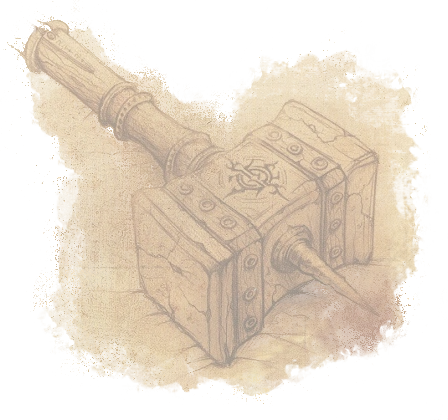
\includegraphics[width=1.3\columnwidth]{%
		images/Magic_Items/Hammer_of_Glory_background.png%
	}};%
\end{tikzpicture}%
	
\section*{Appearance}
{\entryfont The Hammer of Glory is a magnificent artifact, its design radiating both power and elegance. The head is crafted from a mysterious material described in legend as a "crystal enchantment of steel." This silvery-gray metal shimmers with a faint iridescence, occasionally catching the light in soft hues of blue. Its surface is adorned with glowing runes and intricate patterns, pulsing faintly as if alive with hidden magic.

The handle is formed from ancient dark wood, its grain polished smooth with age, reinforced by intricately engraved golden bands that add both strength and beauty. Balanced and proportional, the hammer feels both ceremonial and deadly, crafted for a hero of unmatched purpose. Surrounding it is a faint, golden aura, imbuing the artifact with a quiet majesty that commands reverence. Its presence exudes a restrained power, hinting at its potential to shape both battle and destiny.}

\section*{History}
{\entryfont The Hammer of Glory is one of the legendary Three Relics of Legends, an extraordinary trio of artifacts that includes the Knife of Evil and the Vorpal Laserblaster of Pittenweem. Crafted eons ago by the enigmatic Starlords, these relics were forged to combat an ancient, unknowable evil that threatened the cosmos in the year 10,000 BD.

Wielded during this monumental conflict, the Hammer of Glory became a symbol of defiance and hope, its power instrumental in turning the tide of battle. Once the evil was vanquished, the Starlords, fearing the potential misuse of the relics, made the decision to hide them away. The Hammer of Glory was concealed on Earth, buried deep within the rugged Cairngorm Mountains in what is now Scotland.

To this day, the Hammer of Glory remains hidden, its exact location a mystery. No map or record was left behind, and the Starlords ensured that its resting place would be inaccessible to any but the most determined and worthy.}

\section*{Magic}
{\entryfont The Hammer of Glory is a weapon of unparalleled power, its magic fueled by raw solar energy. The artifact seems to draw strength directly from the sun, radiating an intense, golden light that grows stronger when bathed in sunlight. This celestial energy not only enhances the hammer's durability and destructive force but also imbues it with a radiant aura that inspires allies and strikes fear into foes.

Only a warrior "with a heart pure of steel" can wield the Hammer of Glory. This enigmatic requirement speaks to both moral integrity and unshakable resolve, rejecting any who lack the strength of spirit or character necessary to command its immense power. To its chosen wielder, the hammer grants the ability to kill even immortal beings, severing their existence in defiance of natural or supernatural laws.

The Hammer of Glory also channels its wielder's fury into devastating enchantments. When its power is unleashed, it can focus this wrath into a concussive force that causes enemies' heads to "explode with fury", an effect both terrifying and unstoppable.}

\subsection*{Gameplay Mechanics}
{\entryfont The Hammer of Glory holds a number of charges equal to the value listed for each state. It regains all expended charges during a Long Rest.
\subsubsection*{Dormant State}
\textbf{Charges: 1}
\begin{itemize}
	\item The wielder gains a +1 bonus to attack and damage rolls made with this weapon.
	\item As an action, the wielder can expend 1 charge to channel the hammer's power in a concussive wave of force. Each creature of their choice within a 5-foot radius must succeed on a Dexterity saving throw or take 2d6 force damage. On a success the creature takes half the amount. The Saving Throw DC is calculated as follows:
\end{itemize}
\begin{center}
	\textbf{DC = 8 + Proficiency Bonus + Strength Modifier}
\end{center}
\paragraph*{Awaken}
\subsubsection*{Awakened State}
\textbf{Charges: 4}
\begin{itemize}
	\item The bonus to attack and damage rolls increases to a +2.
	\item The damage of the concussive wave increases to 3d6 and the radius to 10 feet.
	\item The wielder  can expend 3 charges as an action to shatter a Wall of Force as if using the Disintegrate spell.
\end{itemize}
\paragraph*{Exalt}
\subsubsection*{Exalted State}
\textbf{Charges: 7}
\begin{itemize}
	\item The bonus to attack and damage rolls increases to a +3.
	\item The damage of the concussive wave increases to 4d6.
\end{itemize}}